\documentclass[12pt, 
hyperref={colorlinks=true, linkcolor=blue, urlcolor=cyan}]{beamer}
\usetheme{default} 

\setbeamertemplate{navigation symbols}{} %gets rid of navigation symbols
\setbeamertemplate{footline}{} %gets rid of bottom navigation bars
\setbeamertemplate{footline}[page number]{} %use this for page numbers

\setbeamertemplate{itemize items}[circle] %round bullet points
\setlength\parskip{10pt} % white space between paragraphs

\usepackage{wrapfig}
\usepackage{subfig}
\usepackage{setspace}
\usepackage{enumerate}
\usepackage{graphicx}
\usepackage{amsmath}
\usepackage{amsfonts}
\usepackage{amssymb}
\usepackage{amsthm}
\usepackage[UKenglish]{isodate}
\usepackage{verbatim}
\cleanlookdateon

% the preamble
\title{BIOST 311: \\ Regression Methods for the Health Sciences}
\author{Kelsey Grinde and Brian Williamson}
\institute{UW Biostatistics}
\date{Spring 2018}

\begin{document}
% title slide
\begin{frame}
\titlepage\thispagestyle{empty}
\end{frame}

% make it 1.something
\setbeamertemplate{footline}{%
  \raisebox{5pt}{\makebox[\paperwidth]{\makebox[120pt]{\scriptsize Last updated \today}\hfill\makebox[10pt]{\scriptsize 1.\insertframenumber~~}}}}  \newcounter{chap1}{\value{1}}
\setcounter{framenumber}{\value{chap1}}

\begin{frame}
\frametitle{CHAPTER 1: LINEAR REGRESSION}
By the end of Chapter 1, you should be able to: \vspace{-0.3cm}

\begin{itemize}
\item Formulate a regression model, given a scientific or statitical question
\item Interpret the coefficients for a (simple or multiple) linear regression model
\item Interpret confidence intervals and p-values for linear regression coefficients
\item Classify variables according to their role in a linear regression model (e.g., outcome, predictor, potential confounder, effect modifier, precision variable)
\item Use \texttt{R} to fit a linear regression model (and know where in the output to look for the information we need to interpret results)
\item Create graphs to support your linear regression analysis
\end{itemize}

\end{frame}

\section{Simple Linear Regression}
\begin{frame}
\frametitle{SECTION 1: SIMPLE LINEAR REGRESSION}

\center 
\color{red} \begin{large} $y = a + bx$ \end{large} 

\vspace{-0.2cm} 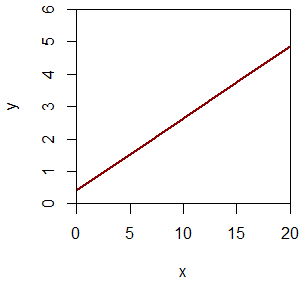
\includegraphics{./plots/plot_y_vs_x}

\end{frame}

% y = a + bx interpretation
\begin{frame}
\frametitle{Determining the slope and intercept of a line}

\center
\begin{large} \color{red} $y = a + bx$ \end{large} \color{black}: \textit{What is a? What is b?}

\vspace{-0.2cm} 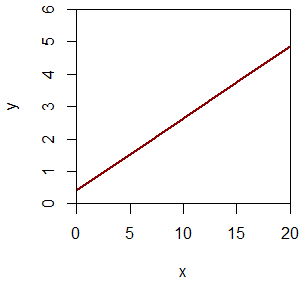
\includegraphics{./plots/plot_y_vs_x} % practice on this example, write interpretation on white board (to come back to)

\end{frame}

% FEV vs age example
\begin{frame}
\frametitle{Simple linear regression}

\center
\begin{large} \color{red} $E[Y|X] = \beta_0 + \beta_1 X$ \end{large} 

\vspace{-0.2cm} 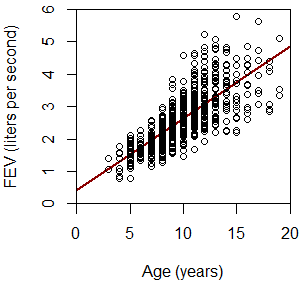
\includegraphics{./plots/plot_fev_vs_age}

\end{frame}

% what is linear regression
\begin{frame}
\frametitle{Simple linear regression}

\begin{center} 
 \color{red} $E[Y|X] = \beta_0 + \beta_1 X$ \color{black}
\end{center} \vspace{-0.3cm}

\begin{small} \textit{Let's take our data and fit the ``best" line through it. That line models the average outcome $Y$ (e.g., FEV), given the predictor $X$ (e.g., age), as a linear function of $X$ (e.g., age).} \end{small}

\center
\vspace{-0.3cm} \center 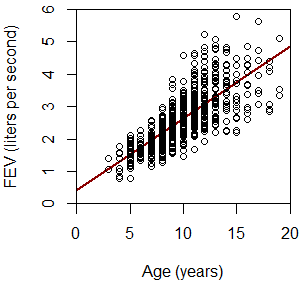
\includegraphics[height=0.65\textheight]{./plots/plot_fev_vs_age}

\end{frame}

% explain linear regression notation
\subsection{Regression Model Notation}
\begin{frame}
\frametitle{Simple linear regression: notation and terminology}
$$\color{blue} E[Y|X] \color{black} = \color{orange} \beta_0 \color{black} + \color{red} \beta_1 \color{yellow} \ X$$ \vspace{-0.6cm}

\color{blue}The average of the response, given the value of the predictor, \color{black} is \color{orange} the intercept \color{black} plus \color{red} the slope \color{black} times \color{yellow} the value of the predictor.\color{black} \pause

\vspace{-0.2cm}
\begin{itemize}
\item $Y$ = outcome, response
\item $X$ = exposure, predictor \pause
\item $E[Y] =$ expected value =  mean of $y$ in the population \pause
\item $E[Y|X]$ = conditional expectation = population mean of $Y$, given information about $X$	\pause
\item Examples: $Y$ is height, $X = 1$ if female and $0$ if male
	\begin{itemize}
	\item $E[Y]$ = 67.1" (the average height in the population)
	\item $E[Y|X = 0]$ = 69.7" (the average height of males)
	\item $E[Y|X = 1]$ = 64.6" (the average height of females)
	\end{itemize}
\end{itemize}
\end{frame}

% interpreting slope and intercept
\subsection{Interpreting Regression Coeffients}
\begin{frame}
\frametitle{Simple linear regression: interpretation}

The \textit{coefficients} ($\beta_0$,$\beta_1$) in our simple linear regression model $E[Y|X] = \beta_0 + \beta_1 X$ often have useful interpretations.

Let's start with the intercept, $\beta_0$: \textit{how would you interpret this coefficient?} \vspace{-0.3cm}
\begin{itemize}
\item[] (Hint: think about how we interpret $a$ in $y=a+bx$)\pause 
\item[] \color{blue} $\beta_0$ is the mean value of $Y$ among subjects with $X = 0$ \color{black}
\end{itemize}

And now the slope, $\beta_1$: \textit{how would you interpret this coefficient?} \vspace{-0.3cm}
\begin{itemize}
\item[] (Hint: think about how we interpret $b$ in $y=a+bx$) \pause
\item[] \color{blue} $\beta_1$ is the difference in mean value of $Y$ comparing two groups that differ in $X$ by one unit \color{black}
\end{itemize}

\end{frame}

% practice: interpreting intercepts
\begin{frame}
\frametitle{Practice: interpreting intercepts in context}

\begin{center} $E[\text{FEV} | \text{age}] = 0.43 + 0.22 \times \text{age}$ \end{center} 

\vspace{-0.3cm} Which of these is correct? \vspace{-0.3cm}
\begin{enumerate}
\item A child with age = $0$ will have FEV equal to 0.43 liters per second
\item Among all children of age 0, the average FEV is 0.43 liters per second \vspace{-0.2cm}
\end{enumerate} \pause

\color{red} Questions to consider when interpreting intercepts: \vspace{-0.3cm} \color{black}
\begin{itemize}
\item \textit{What is the scientific interpretation of ``children with age = 0``? Does our intercept make scientific sense?} \\ \pause  % Yes, age = 0 <--> birth
\item \textit{What if I replaced age with height in the formula above?} \\ \pause % No, height = 0 <-- DNE\
\item \textit{What if we did this study on adults (ages 40--60), and got the same intercept? Would you trust the intercept?} %% No! Be careful not to extrapolate too far beyond range of data
\end{itemize}

\end{frame}

% practice: interpreting slopes
\begin{frame}
\frametitle{Practice: interpreting slopes in context}

\begin{center} $E[\text{FEV} | \text{age}] = 0.43 + 0.22 \times \text{age}$ \end{center} 

\textit{What is the difference between these two interpretations?} \vspace{-0.3cm}
\begin{itemize}
\item For every one year increase in age, average FEV increases by 0.22 liters per second
\item Comparing two groups of children that differ in age by one year, the difference in average FEV will be 0.22 liters per second, with higher average FEV in the older of the two groups
\end{itemize} \pause

\textit{Which do you think is correct?} \vspace{-0.3cm} \pause 
\begin{itemize}
\item[] (Hint: this was an observational study)
\end{itemize}

% give a couple examples, some with interpretations that are ``too causal"
\end{frame}

% why do we care about the slope?
\begin{frame}
\frametitle{Why do we care about the slope?}

\begin{small} \textit{In which example(s) is there \textbf{no} association between FEV and age?} \vspace{-0.6cm} \end{small}

\hspace*{-0.6cm} 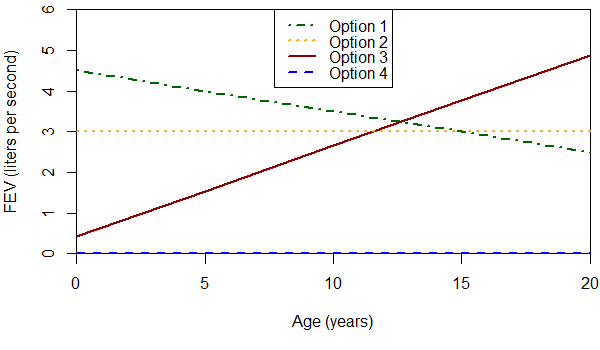
\includegraphics[width=0.9\paperwidth]{./plots/association}

\pause
 \vspace{-0.7cm} \textit{What is the slope in those cases?}
\end{frame}

\begin{frame}
\frametitle{Why do we care about the slope?}

When... \\
$\beta_1 = 0$: there is no linear association between $X$ and $Y$ \\
$\beta_1 > 0$: there is a positive linear association between $X$ and $Y$ \\
$\beta_1 < 0$: there is a negative linear association between $X$ and $Y$

\pause
Suppose we have a \textbf{scientific question:} \textit{is there an association between lung function and age?}

We can use linear regression to answer this question: \vspace{-0.3cm}
\begin{enumerate}
\item Fit the model $E[FEV|age] = \beta_0 + \beta_1 \times age$
\item Check whether or not $\beta_1 = 0$ \color{blue} (estimate, CI, p-value) \color{black}
\end{enumerate}

\pause
What \textbf{statistical question} are we answering? \textit{Is there an association between FEV and age, where association is quantified by difference in mean FEV between age groups}

\end{frame} 


% math explaining slope interpretation
\begin{frame}
\frametitle{Interpreting slopes: mathematical explanation}

For a regression model $E[Y|X] = \beta_0 + \beta_1 X$, \color{blue} we interpret the slope $\beta_1$ as the difference in mean value of $Y$ for two groups differing in $X$ by one unit. \color{black}

Why is this true?
\begin{itemize}
\item $E[Y|X = x] = \beta_0 + \beta_1 x$ \pause
\item $E[Y|X = (x+1)] = \beta_0 + \beta_1(x+1) = \beta_0 + \beta_1 x + \beta_1$ \pause
\item $E[Y|X = (x+1)] - E[Y|X = x] = \beta_1$
\end{itemize}

\end{frame}

% end of Wednesday lecture
\begin{frame}
\frametitle{What's next?}

\begin{itemize}
\item Confidence intervals and hypothesis tests for regression parameters
	\begin{itemize}
	\item \color{blue} Please read the confidence intervals analogy handout and come prepared to discuss on Friday \color{black}
	\end{itemize}
\item What it means to find the line of ``best" fit
\item Using \texttt{R} to fit linear regression models 
\end{itemize}

\end{frame}

% start of Friday lecture
\begin{frame}
\frametitle{Statistical inference: linear regression}

\color{blue} What do we know so far? \color{black}% interpreting coefficients; distinguish between truth and estimate
\begin{itemize}
\item \textbf{Estimate/statistic:} estimated regression coefficient
\item[] (After Wednesday, we know how to interpret. Today we'll talk about how to calculate.)
\end{itemize}

\color{blue} What's missing? \color{black}\pause %ask them about the 4 numbers we always want them to report
\begin{itemize}
\item \textbf{Quantifying uncertainty:} 95\% confidence interval for regression coefficient
\item \textbf{Hypothesis test:} p-value for regression coefficient \pause
\item \textit{What types of scientific questions can we answer using linear regression?}
\item \textit{How do I do all this in R?}
\end{itemize}

\end{frame}


% standard errors
\subsection{Confidence intervals for regression coefficents}
\begin{frame}
\frametitle{Quantifying uncertainty: standard errors (SEs)}

When we estimate regression coefficients, we also want to quantify the \color{blue} uncertainty \color{black} in these estimates.\vspace{-0.2cm} \pause

Just like we have two options for two-sample t-tests (\textit{equal} or \textit{unequal} variances), we have \color{blue} two options for calculating standard errors of regression coefficients\color{black}: \vspace{-0.3cm} \pause
\begin{itemize}
\item \textbf{Naive standard errors}: assume that the population variance of $Y$ is the same across all values of $X$ % assume homoskedasticity
	\begin{itemize}
	\item Only appropriate if this assmption is true
	\item We have no way of knowing if this assumption is true
	\end{itemize}
\item \textbf{Robust standard errors}: allow the population variance of $Y$ to differ across values of $X$ % allow for heteroskedasticity
	\begin{itemize}
	\item Appropriate if the variances differ, or if they're constant!
	\end{itemize}
\end{itemize}
\end{frame}

% picture explaining homoskedasticity vs heteroskedasticity
\begin{frame}
\frametitle{Constant vs non-constant variance}

If we sample from a population with constant variance versus non-constant variance, what does this look like?
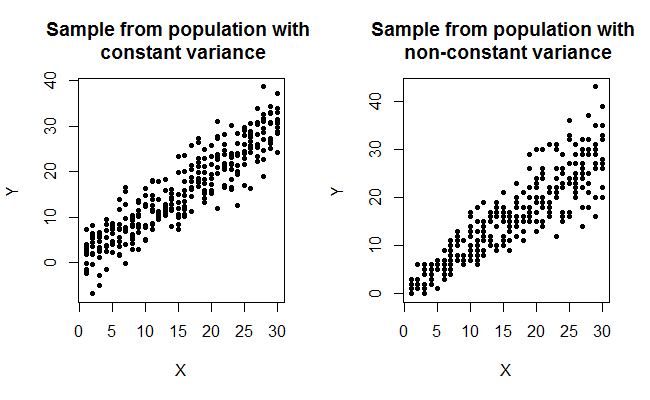
\includegraphics[width=\textwidth]{./plots/hetero}

\end{frame}

\begin{frame}
\frametitle{Choosing between naive and robust SEs}

Naive SEs assume that variance in $Y$ is constant across all values of $X$. Robust SEs are appropriate if variance is constant, or if it's non-constant!

\color{blue} Important: \color{black} what matters is whether the variance is constant \textit{in the population}, which we can't tell by looking at our data.

\color{blue} Conclusion: \color{black} unless you have a very solid scientific reason for variance being constant, use robust SEs.

\color{red} Warning: \color{black} Most software (inappropriately) uses \textit{naive} SEs, but the \texttt{uwIntroStats} package gives us \textit{robust} SEs. % they don't need to know how to calculate, just need to know where to look in regress output

\begin{footnotesize} \textit{Note: the decision about which two-sample t-test to use (equal or unequal variances) relies on a similar thought process} \end{footnotesize}
\end{frame}


% confidence intervals
\begin{frame}
\frametitle{Quantifying uncertainty: 95\% confidence intervals}

Once we have our standard error, we can calculate a 95\% confidence interval. 

Again, there are two options: \vspace{-0.3cm}
\begin{itemize}
\item $\hat{\beta} \pm 1.96 \times \widehat{SE}(\hat\beta)$
\item $\hat{\beta} \pm t_{n-2} \times \widehat{SE}(\hat\beta)$
	\begin{itemize}
	\item If $n = 10, t_{n-2} = 2.31$
	\item If $n = 100, t_{n-2} = 1.98$
	\item If $n = 1000, t_{n-2} = 1.96$
	\end{itemize}
\end{itemize}

Most software (including \texttt{uwIntroStats}) gives you the $t$-based confidence interval. When $n$ is large, there's little difference. Either way, our interpretation remains the same.

% differences between the two come from thinking about what the sampling distribution of \hat\beta is... when n is large, CLT tells us it's normal so first is good; when data are normal, \hat\beta-mu/se is t, for small or large n; in practice: t-intervals work fine in either setting because they're always wider -- may have more than 95% coverage
\end{frame}

\begin{frame}
\frametitle{Interpreting 95\% confidence intervals}

Suppose we use linear regression to evaluate the association between FEV and age, and we estimate the slope to be 0.22, with 95\% confidence interval (0.20, 0.24).

To interpret the CI for a regression coefficient: same language as CI for the mean (0.50) or difference in means (0.60, HW2)

\textit{We estimate that the difference in mean FEV comparing two groups of children that differ by one year in age is 0.22 liters per second, with higher average FEV in the older of the two groups. \color{blue} Based on a 95\% confidence interval, this estimated difference would not be judged unusual if the true difference were between 0.20 and 0.24 liters per second. \color{black}}
\end{frame}

% discussion of CI interpretation dice rolling anlogy
\begin{frame}
\frametitle{Interpreting confidence intervals: rolling the dice}

\textbf{Rolling dice}:\vspace{-0.3cm}
\begin{itemize}
\item \textit{What's random?} The process of rolling
\item Once we've rolled, there's no randomness left, and any probabilites are 0 or 1 (depending on the truth)
\end{itemize}

\pause
\textbf{Estimating quantities from data}:\vspace{-0.3cm}
\begin{itemize}
\item \textit{What's random?} The process of collecting data
\item Once we've collected data, there's no randomness left, and any probabilites are 0 or 1 (depending on the truth)
\end{itemize}

\pause
\begin{small}
Recall the definition of \textbf{probability}: the relative frequency of an event in the long run (i.e., if an experiment is repeated many times, what proportion of those times does the event occur?)\\ \pause
\color{blue} Example: \color{black} If I repeat the process of collecting data many times, and every time check if our \textit{original} confidence interval (0.20,0.24) contains the true difference in means, how often will this happen?\\ \pause \hfill \color{red} Always, or never.
\end{small}

\end{frame}

% back to road map
\begin{frame}
\frametitle{Back to our linear regression roadmap...}
\color{blue} What do we know so far? \color{black}% interpreting coefficients; distinguish between truth and estimate
\begin{itemize}
\item \textbf{Estimate/statistic:} estimated regression coefficient
\item[] (After Wednesday, we know how to interpret. Today we'll talk about how to calculate.)
\end{itemize}

\color{blue} What's missing? \color{black} %ask them about the 4 numbers we always want them to report
\begin{itemize}
\item \textbf{Quantifying uncertainty:} 95\% confidence interval for regression coefficient
\item \textbf{Hypothesis test:} p-value for regression coefficient 
\item \textit{What types of scientific questions can we answer using linear regression?}
\item \textit{How do I do all this in R?}
\end{itemize}
\end{frame}

\begin{frame}[noframenumbering]
\frametitle{Back to our linear regression roadmap...}
\color{blue} What do we know so far? \color{black}% interpreting coefficients; distinguish between truth and estimate
\begin{itemize}
\item \textbf{Estimate/statistic:} estimated regression coefficient
\item \textbf{Quantifying uncertainty:} 95\% confidence interval for regression coefficient
\end{itemize}

\color{blue} What's missing? \color{black} %ask them about the 4 numbers we always want them to report
\begin{itemize}
\item \textbf{Hypothesis test:} p-value for regression coefficient 
\item \textit{What types of scientific questions can we answer using linear regression?}
\item \textit{How do I do all this in R?}
\end{itemize}
\end{frame}

% hypothesis tests
\subsection{Hypothesis tests for regression coefficents}
\begin{frame}
\frametitle{Hypothesis tests}

$$\text{Regression Model: } E[Y|X] = \beta_0 + \beta_1 X$$

Recall that $\beta_1$ quantifies the association between $X$ and $Y$.

To test whether there is a \textit{statistically significant} association between $X$ and $Y$, \color{blue} we just need to test whether $\beta_1 = 0$: \vspace{-0.3cm} \color{black}
\begin{itemize}
\item $H_0: \beta_1 = 0$
\item $H_1: \beta_1 \not= 0$
\end{itemize}

\pause
Interpret the $p$-value just as before! (e.g., 0.59--0.60, HW2) \vspace{-0.4cm}
\begin{small}
\begin{itemize} \itemsep -2pt
\item $p < \alpha$: \textbf{reject $H_0$}, ``we have evidence to suggest that $X$ is associated with $Y$"
\item $p > \alpha$: \textbf{fail to reject $H_0$}, ``we do not have enough evidence to support the hypothesis that $X$ is associated with $Y$"
\end{itemize}
\end{small}
\end{frame}

% putting it in context: from scientific question to conclusions (FEV vs age)
\subsection{From scientific question to conclusions: continuous predictor}
\begin{frame}
\frametitle{Example: lung function and age}

\begin{enumerate}
\item \textbf{Scientific question:} is \color{blue} lung function \color{orange} associated \color{black} with age among US children? \pause
\item \textbf{Statistical question:} is there a \color{orange} difference in average \color{blue} FEV \color{black} comparing groups of US children that differ in age? \pause
	\begin{itemize}
	\item \textbf{Population:} all US children
	\item \textbf{Parameter:} population linear regression slope (diff. in means comparing groups that differ by one year in age) \pause
	\end{itemize}
\item Take a \textbf{sample} from the population: 654 children who came into a pediatric clinic for a routine check-up \pause
\item Perform \textit{statistical inference}:
	\begin{itemize}
	\item Calculate the corresponding \textbf{statistic}: sample linear regression slope (estimated difference in means comparing groups that differ by one year in age) \pause
	\item Quantify the uncertainty in your statistic
	\item Perform a hypothesis test \pause
	\end{itemize}
\item Make conclusions in context of original questions
\end{enumerate}

\end{frame}

% show R output
\begin{frame}
\frametitle{Example: lung function and age}
To fit the regression model \color{blue} $E[\text{FEV}|\text{age}] = \beta_0 + \beta_1 \text{ age}$ \color{black} in \texttt{R}:\\ (1) load \texttt{uwIntroStats}, (2) use the \texttt{regress} function. \vspace{-0.3cm}

\center
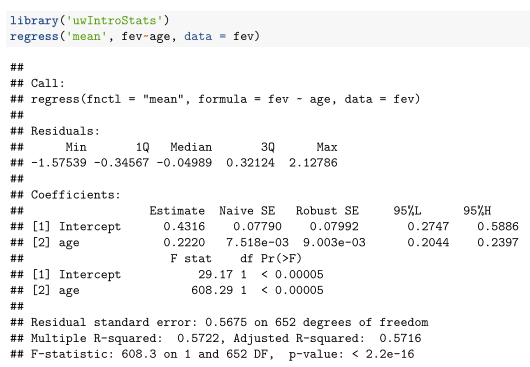
\includegraphics[width=0.55\paperwidth]{./plots/regress_fev_vs_age}
\end{frame}

% highlight what's important
\begin{frame}
\frametitle{Example: lung function and age}
Which pieces do we need to answer our question about the association between FEV and age? \vspace{-0.3cm}

\center
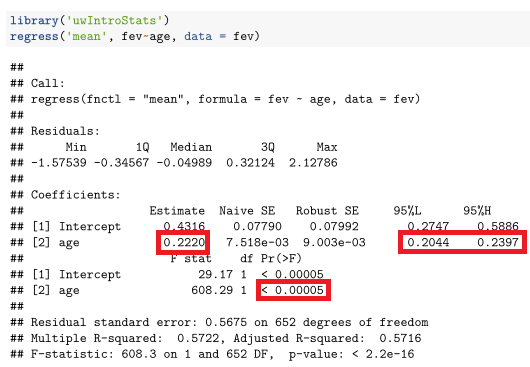
\includegraphics[width=0.55\paperwidth]{./plots/regress_fev_vs_age_highlights}
\end{frame}

% interpret results
\begin{frame}
\frametitle{Example: lung function and age}
Interpreting our results:\vspace{-0.3cm}
\begin{itemize}
\item \textit{Statistic:} We estimate that the difference in mean FEV comparing two groups of children that differ by one year in age is 0.22 liters per second, with higher average FEV in the older of the two groups. \pause
\item \textit{Uncertainty:} Based on a 95\% confidence interval, this estimated difference would not be judged unusual if the true difference were between 0.20 and 0.24 liters per second.\pause
\item \textit{Hypothesis test p-value:} These data provide strong evidence that the difference in mean FEV between groups of children that differ by one year in age is significantly different from zero (p $<$ 0.001). \pause
\item \textit{Conclusion:} These data provide evidence to suggest that older children tend to have higher FEV. 
\end{itemize}
\end{frame}

% new example: binary predictor
\begin{frame}
\frametitle{Example: lung function and age}
\textit{Why haven't we said anything about the intercept?} \pause
\begin{itemize}
\item Interpretation: We estimate that the average FEV among newborns is 0.22 L/sec \pause
\item But... 
	\begin{itemize}
	\item \textit{Is this scientifically relevant?} Maybe not.
	\item Most importantly, \color{blue} the intercept has nothing to do with our scientific question \color{black} (is FEV associated with age?) \pause
	\end{itemize}
\item Since the intercept is not relevant to our primary scientific question, we don't care about the CI or p-value
\end{itemize}
\end{frame}


% putting it in context: from scientific question to conclusions (FEV vs sex) = special case with binary predictor
%%%% if time: use genetics example instead
\subsection{From scientific question to conclusions: binary predictor}
\begin{frame}
\frametitle{Example: lung function and sex}

\begin{enumerate}
\item \textbf{Scientific question:} do boys and girls (in the US) have different lung function?
\item \textbf{Statistical question:} is there a difference in average FEV between boys and girls in the US?
\end{enumerate} 

Earlier this week, we used the two-sample t-test (with unequal variances) to address this question.

We can also use linear regression!
\end{frame}

% show R output
\begin{frame}
\frametitle{Example: lung function and sex}
To fit the regression model \color{blue} $E[\text{FEV}|\text{male}] = \beta_0 + \beta_1 \text{ male}$ \color{black} in \texttt{R}:\\ (1) load \texttt{uwIntroStats} (not shown here), (2) re-code \texttt{sex} to create a binary variable \texttt{male}, and (3) run \texttt{regress}. \vspace{-0.5cm}

\center
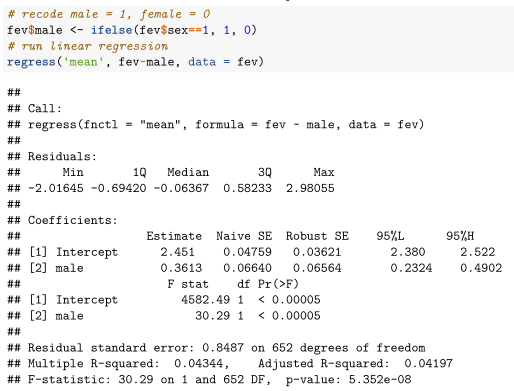
\includegraphics[width=0.6\paperwidth]{./plots/regress_fev_vs_sex}

\end{frame}

\begin{frame}
\frametitle{Example: lung function and sex}

Our linear regression results:

\begin{itemize}
\item \textit{Statistic:} We estimate that the difference in mean FEV between girls and boys is 0.361 liters per second (with boys tending to have the higher mean FEV). \pause
\item \textit{Uncertainty:} Based on a 95\% confidence interval, this observed difference would not be judged unusual if the true difference were between 0.232 and 0.490 liters per second.\pause
\item \textit{Hypothesis test p-value:} These data provide strong evidence that the difference in mean FEV between groups is different from zero (p $<$ 0.001).\pause
\item \textit{Conclusion:} These data provide evidence to suggest that male children tend to have higher FEV.
\end{itemize}

\end{frame}

\begin{frame}
\frametitle{Example: lung function and sex}

Our t-test results: 

\begin{itemize}
\item \textit{Statistic:} We estimate that the difference in mean FEV between girls and boys is 0.361 liters per second (with boys tending to have the higher mean FEV). 
\item \textit{Uncertainty:} Based on a 95\% confidence interval, this observed difference would not be judged unusual if the true difference were between 0.232 and 0.490 liters per second.
\item \textit{Hypothesis test p-value:} These data provide strong evidence that the difference in mean FEV between groups is different from zero (p $<$ 0.001).
\item \textit{Conclusion:} These data provide evidence to suggest that sex is associated with FEV in children.
\end{itemize}

\end{frame}

\begin{frame}
\frametitle{Example: lung function and sex}

\begin{itemize}
\item \color{blue} If you use linear regression with a binary predictor, this is essentially the same as performing a two-sample t-test \color{black}
	\begin{itemize}
	\item Difference in mean between groups differing by one unit (for a binary predictor, you can only differ by one unit)
	\end{itemize}
\item If you use naive SEs, this is \textit{exactly} equivalent to the t-test which presumes equal variances
\item If you use robust SEs, this is \textit{approximately} equivalent\footnote[frame]{Our results look exactly the same, but if you go out to more digits you see slight differences in, e.g., the CI: (0.23235, 0.49020) and (0.23238, 0.49017) for the t-test and linear regression, respectively\\} to the t-test which allows for unequal variances
\end{itemize}

\vspace{-0.2cm} No matter your choice of SEs, your estimates will be the same: $\beta_1$ = the differences in means, $\beta_0 = $ the mean in ``group 0"


\end{frame}

% "Under the hood" -- how do we get a linear regression line?
%%% explain ideas behind least squares estimation
\subsection{Under the hood: least squares estimation}
\begin{frame}
\frametitle{Least squares estimation}
What is \texttt{R} doing \textit{under the hood} to get these regression coefficient estimates?\vspace{-0.6cm} \pause 

\center 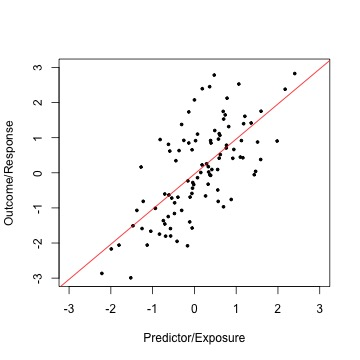
\includegraphics[height=0.7\textheight]{./plots/linear-regr}
\end{frame}

\begin{frame}
\frametitle{Least squares estimation}
\textit{Least squares:} minimize the sum of the squared distances from the observed points to the fitted line.\vspace{-0.6cm}

\center 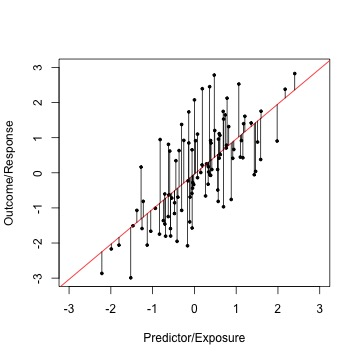
\includegraphics[height=0.7\textheight]{./plots/linear-regr-ls}
\end{frame}

\begin{frame}
\frametitle{Least squares estimation: technical details}
\textit{Least squares:} minimize the sum of the squared distances from the observed points to the fitted line. \pause

We can write this as an optimization problem, $$ \text{argmin}_{\beta_0,\beta_1} \sum_{i=1}^n \left(Y_i - \left[\beta_0 + \beta_1 X_i\right]\right)^2,$$ \pause which has a closed form solution:\vspace{-0.3cm}
\begin{itemize}
\item $\hat\beta_1 = \frac{\sum_i \left(X_i - \bar{X}\right)\left(Y_i - \bar{Y}\right)}{\sum_i \left(X_i - \bar{X}\right)^2}$
\item $\hat\beta_0 =\bar{Y} - \hat\beta_1 \bar{X}$
\end{itemize}

\center \color{blue} \textit{You will \textbf{NOT} be tested on these!} \color{black}
\end{frame}

\subsection{Regression and correlation}
% aside: connect to correlation
\begin{frame}
\frametitle{Simple linear regression and correlation}

Notice how much our slope estimate looks like Pearson's correlation ($r$): 
$$\hat\beta_1 = \frac{\sum_i \left(X_i - \bar{X}\right)\left(Y_i - \bar{Y}\right)}{\sum_i \left(X_i - \bar{X}\right)^2}$$
$$r = \frac{\sum_i \left(X_i - \bar{X}\right)\left(Y_i - \bar{Y}\right)}{\sqrt{\sum_i\left(X_i - \bar{X}\right)^2} \sqrt{\sum_i \left(Y_i - \bar{Y}\right)^2}}$$ \pause

\begin{itemize}\vspace{-0.3cm}
\item $\hat\beta_1$ and $r$ have the same sign: both positive, both negative, or both zero
\item Testing $H_0: r = 0$ is equivalent to testing $H_0: \beta_1 = 0$
\item $\hat\beta_1$ has a more meaningful (and scientifically relevant) interpretation
\item (Coming soon:) Linear regression also lets us adjust for other variables; correlation does not
\end{itemize}

\end{frame}


\begin{frame}
\frametitle{Index Card \# 3}

\begin{enumerate}
\item Name
\item Something you learned this week.
\item Something you \textit{were} struggling with/had questions about, but now feel more confident about.
\item Something you \textit{are} struggling with/have questions about.
\item Does our office hours time (Wed, 2--4) work for you?
\item Have you ever used Poll Everywhere?
\end{enumerate}

\end{frame}

%% start here 4/9
\begin{frame}
\frametitle{Linear regression roadmap}
\color{blue} What do we know so far? \color{black}\vspace{-0.3cm}% interpreting coefficients; distinguish between truth and estimate
\begin{itemize}
\item \textbf{Estimate/statistic:} estimated regression coefficient
\item \textbf{Quantifying uncertainty:} 95\% confidence interval for regression coefficient
\item \textbf{Hypothesis test:} p-value for regression coefficient 
\item \textit{What types of scientific questions can we answer using linear regression?}
	\begin{itemize}
	\item Continuous outcome vs continuous predictor
	\item Continuous outcome vs binary predictor
	\end{itemize}
\item \textit{How do I do all this in R?} (and what R is doing)
\end{itemize}

\color{blue} What's next?\vspace{-0.3cm}
\begin{itemize}
\item Transforming our predictor or outcome
\item Linear regression with a categorical predictor
\end{itemize}
\end{frame}

\subsection{Transformations}
% Warm-up activity: FEV vs age
\begin{frame}
\frametitle{Interpreting coefficients (no transformation)}
How do we interpret $\beta_0, \beta_1$ in this linear regression model? $$E[\text{FEV}|\text{Age}] = \beta_0 + \beta_1 \text{Age}$$

$\beta_0$: average value of $Y$ among subjects with $X = 0$ \\ \pause
\ \ \ \ \ \color{blue} average FEV (l/sec) among newborns \color{black} \pause

$\beta_1$: difference in average value of $Y$ comparing two groups that differ in $X$ by one unit\\ \pause
\ \ \ \ \ \color{blue} difference in average FEV (l/sec) comparing two groups that differ in age by one year 
\end{frame}

% Warm-up activity: Age+3
\begin{frame}
\frametitle{Interpreting coefficients after a transformation}
How do we interpret $\beta_0$ in this linear regression model? $$E[\text{FEV}|\color{blue}(\text{Age}-3)\color{black}] = \beta_0 + \beta_1 \color{blue}\left(\text{Age}-3\right)\color{black}$$

\vspace{-0.5cm}
$\beta_0$: average value of $Y$ among subjects with $X = 0$ \\ \pause
\ \ \ \ \ average FEV (l/sec) among kids with $\text{Age} -3 = 0$\\ \pause
\ \ \ \ \ \color{blue} average FEV (l/sec) among 3 year olds \color{black} \pause

Why are those last two interpretations equivalent?
\begin{align*}
(\text{Age}-3) &= 0 \\ 
\text{Age} &= 3
\end{align*}
\end{frame}

% Age-3: slope
\begin{frame}
\frametitle{Interpreting coefficients after a transformation}
How do we interpret $\beta_1$ in this linear regression model? $$E[\text{FEV}|(\text{Age}-3)] = \beta_0 + \beta_1 \left(\text{Age}-3\right)$$

\vspace{-0.5cm}
$\beta_1$: difference in average value of $Y$ comparing two groups that differ in $X$ by one unit\\ \pause
\ \ \ \ \ difference in average FEV (l/sec) comparing two groups that differ in $\text{Age}-3$ by one year\\ \pause
\ \ \ \ \ \color{blue} difference in average FEV (l/sec) comparing two groups that differ in age by one year \color{black}\pause

Why are those last two interpretations equivalent?
\begin{align*}
(\text{Age}-3) = x+1 &\color{red} \text{ vs } \color{black} (\text{Age}-3) = x \\
\text{Age} = x+4 &\color{red} \text{ vs } \color{black} \text{Age} = x+3
\end{align*}
\end{frame}

% Warm-up activity
\begin{frame}
\frametitle{Interpreting coefficients: your turn!}
On a piece of paper, please:\vspace{-0.3cm}
\begin{enumerate} \itemsep +5pt
\item Write your name
\item Interpret\footnote[frame]{\color{blue} Don't forget units! FEV = liters/second, Age = years} $\beta_0, \beta_1$ in the following models:
	\begin{enumerate}\itemsep +5pt
	\item $E[\text{FEV}|\left(\text{Age}-\overline{Age}\right)] = \beta_0 + \beta_1 \left(\text{Age}-\overline{Age}\right)$ 
	\item $E[\text{FEV}|\left(\frac{\text{Age}}{10}\right)] = \beta_0 + \beta_1 \left(\frac{\text{Age}}{10}\right)$ 
	\item $E[\text{FEV}|\left(\frac{\text{Age}-3}{10}\right)] = \beta_0 + \beta_1 \left(\frac{\text{Age}-3}{10}\right)$ 
	\end{enumerate}
\item Interpret $\beta_0, \beta_1$ in the following models:
	\begin{enumerate}\itemsep +5pt
	\item $E[(\text{FEV}\times 60)|\text{Age}] = \beta_0 + \beta_1 \text{Age}$ 
	\item $E[\left(\frac{\text{FEV}}{3.78541}\right)|\text{Age}] = \beta_0 + \beta_1 \text{Age}$ \begin{scriptsize}\\(Hint: 1 gallon = 3.78541 liters)\end{scriptsize}
	\end{enumerate}
\end{enumerate}
\end{frame}

% pause to walk through answers

% motivation for linear transformations
\subsubsection{Linear transformations}
\begin{frame}
\frametitle{Linear transformations of $X$ and $Y$}

\textit{Linear transformations:} adding, subtracting, multiplying, and/or dividing by some constant

Which transformations changed our interpretation of $\beta_0$?\vspace{-0.3cm}\pause
\begin{itemize}
\item[] Adding (subtracting) a constant to (from) $X$
\item[] Any change to $Y$\pause
\end{itemize}

Which transformations changed our interpretation of $\beta_1$?\pause
\vspace{-0.3cm}
\begin{itemize}
\item[] Dividing (multiplying) $X$ by a constant  
\item[] Any change to $Y$
\end{itemize}
\end{frame}

\begin{frame}
\frametitle{Why transform $X$ and/or $Y$?}
Why might we want to transform our variables? 
\begin{itemize}
\item \textit{Make interpretation of $\beta_0$ more scientifically meaningful} (e.g., so we're not talking about the average FEV among people with height 0")
\item \textit{Make estimate of $\beta_0$ more trustworhty} (e.g., so we're not estimating the average FEV among newborns if all our data were collected on senior citizens)
\item \textit{Change units of outcome and/or predictor} (e.g., difference in FEV in liters/minute comparing two groups that differ in age by one year)
\end{itemize}

We'll come back to this...
\end{frame}

% summary of types of transformations they should know
\begin{frame}
\frametitle{Types of transformations}

So far we've seen:
\begin{enumerate}
\item Adding/subtracting a constant (e.g., $\text{Age} - \overline{Age}$)
\item Multiplying/dividing by a constant (e.g., $\text{Age}/10$)
\item A combination of 1. and 2. (e.g., $(\text{Age}-3)/10$)
\end{enumerate}

What other types of transformations might we use?
\begin{enumerate}
\item Log transformations
\item Polynomial transformations (e.g., $x + x^2$)
\end{enumerate}

\end{frame}

\subsubsection{Log transformations}
% log(X) - beta_0
\begin{frame}
\frametitle{Transformations: $\log(X)$}
\begin{center} $E[FEV|\log(\text{Height})] = \beta_0 + \beta_1 \log(\text{Height})$ \end{center}

$\beta_0$: average value of $Y$ among subjects with $X = 0$\\ \pause 
\ \ \ \ \ average FEV among subjects with $\log(\text{Height}) = 0$\\ \pause 
\ \ \ \ \ \color{blue} average FEV among subjects who are 1 inch tall \color{black}  \pause

Why are those last two interpretations equivalent?
\begin{align*}
\log(\text{Height}) & = 0 \\
e^{\log(\text{Height})} & = e^0 \\
\text{Height} & = 1\\
\end{align*}
\begin{footnotesize} Note: in statistics (and in \texttt{R}), when we write $\log$, we mean $\log_e = \ln$ \end{footnotesize}
\end{frame}

% log(X) - beta_1
\begin{frame}
\frametitle{Transformations: $\log(X)$}
\begin{center} $E[FEV|\log(\text{Height})] = \beta_0 + \beta_1 \log(\text{Height})$ \end{center}

$\beta_1$: difference in average value of $Y$ comparing two groups that differ in $X$ by one unit\\ \pause
\ \ \ \ \ difference in average FEV comparing two groups that differ in $\log(\text{Height})$ by one unit\\ \pause
\ \ \ \ \ \color{blue} difference in average FEV comparing two groups that differ in height by a multiplicative factor of $e$ (2.718...) \color{black} \pause

Why are those last two interpretations equivalent?
\begin{align*}
\log(\text{Height}) = x + 1 &\color{red}\text{ vs }\color{black} \log(\text{Height}) = x \\
e^{\log(\text{Height})} = e^{x+1} &\color{red}\text{ vs }\color{black} e^{\log(\text{Height})} = e^x \\
\text{Height} = e^{x}e &\color{red}\text{ vs }\color{black} \text{Height} = e^{x}
\end{align*}
\end{frame}

% log(X) - beta_1
\begin{frame}
\frametitle{Transformations: $\log(X)$}
An $e$-fold difference between two groups is not very intuitive. How can we make our interpretation of $\beta_1$ better?

Option 1: use a different base\pause
\begin{itemize}
\item $E[FEV|\color{blue}\log_2\color{black}(Height)] = \beta_0 + \beta_1 \color{blue}\log_2\color{black}(Height)$
	\begin{itemize}
	\item $\beta_0$: average FEV among subjects who are 1" tall
	\item $\beta_1$: difference in average FEV comparing groups that differ in height by a \color{blue} multiplicative factor of 2\color{black}
	\end{itemize} \pause
\item $E[FEV|\color{blue}\log_{10}\color{black}(Height)] = \beta_0 + \beta_1 \color{blue}\log_{10}\color{black}(Height)$
	\begin{itemize}
	\item $\beta_0$: average FEV among subjects who are 1" tall
	\item $\beta_1$: difference in average FEV comparing groups that differ in height by a \color{blue}multiplicative factor of 10\color{black}
	\end{itemize}
\end{itemize}
\end{frame}

% log(X) - beta_1
\begin{frame}
\frametitle{Transformations: $\log(X)$}
An $e$-fold difference between two groups is not very intuitive. How can we make our interpretation of $\beta_1$ better?

Option 2: fit the same model \begin{scriptsize}($E[FEV|\log(Height)] = \beta_0 + \beta_1\log(Height)$)\end{scriptsize} but interpret $c \times \beta_1$ rather than $\beta_1$ \pause

\textit{Example:} $\color{blue}\log(1.1)\color{black}\beta_1$ is the difference in average FEV comparing two groups that differ in height by a \color{blue}multiplicative factor of 1.1 \color{black} (i.e., a 10\% difference)\pause
	\begin{align*}
	E[FEV|&\log(Height=1.1x)]-E[FEV|\log(Height=x)] \\
	& = \left[\beta_0 + \beta_1\log(1.1x)\right] - \left[\beta_0 + \beta_1 \log(x) \right]\\
	& = \left[\beta_0 + \beta_1\{\log(1.1)+\log(x)\}\right] - \left[\beta_0 + \beta_1 \log(x) \right]\\
	& = \left[\beta_0 + \beta_1\log(1.1)+\beta_1\log(x)\right]-\left[\beta_0 + \beta_1 \log(x) \right]\\
	& = \beta_1\log(1.1)
	\end{align*}
\end{frame}

% summary: log(X)
\begin{frame}
\frametitle{Transformations: $\log(X)$}
Tying it all together...
\begin{itemize}
\item \color{blue} Regression model: \color{black} $E[Y|\log(X)] = \beta_0 + \beta_1\log(X)$
\item \color{blue} $\beta_0$: \color{black} average value of $Y$ among subjects with $X = 1$
\item \color{blue} $\log(k)\times\beta_1$: \color{black} difference in average value of $Y$ comparing two groups that differ in $X$ by a multiplicative factor of $k$
\end{itemize}\pause

Why would we want to do this type of transformation?
\begin{itemize}
\item Sometimes it is more scientifically relevant to talk about multiplicative changes in $X$ rather than differences in $X$
\item Types of variables that we often $\log$ transform:
	\begin{itemize}
	\item Money (e.g., salary, home prices)
	\item Biological measurements (e.g., prostate specific antigen in prostate cancer, serum creatinine in kidney disease)
	\end{itemize}
\end{itemize}
\end{frame}

% log(Y)
\begin{frame}
\frametitle{Transformations: $\log(Y)$}
\begin{center} $E[\log(FEV)|Height] = \beta_0 + \beta_1 Height$ \end{center}
$\beta_0$: average value of $Y$ among subjects with $X = 0$\\ \pause
\ \ \ \ \ average $\log(FEV)$ among subjects that are 0" tall \\ \pause
\ \ \ \ \ log geometric mean FEV among subjects that are 0" tall \\ \pause
\color{blue} $e^{\beta_0}$: geometric mean of FEV among subjects that are 0" tall \color{black}\pause

Why are those interpretations equivalent?\vspace{-0.3cm}
\begin{itemize}
\item[] \textit{Arithmetic mean}: $\frac{1}{n} \sum_{i=1}^n a_i$
\item[] \textit{Geometric mean}: $\left(\prod_{i=1}^n a_i\right)^{\frac{1}{n}} = e^{\frac{1}{n} \sum_{i=1}^n \log(a_i)}$
\end{itemize}
\begin{center} \begin{footnotesize}The ``average of $\log(Y)$" = $\frac{1}{n}\sum \log(Y_i)$ \ \textit{is the same as}\\the ``log of the geometric mean of $Y$" = $\log(e^{\frac{1}{n}\sum \log(Y_i)} = \frac{1}{n}\sum \log(Y_i)$.\end{footnotesize}\end{center}
\end{frame}

%log(Y) - beta_1
\begin{frame}
\frametitle{Transformations: $\log(Y)$}
\begin{center} $E[\log(FEV)|Height] = \beta_0 + \beta_1 Height$ \end{center}
$\beta_1$: difference in average values of $Y$ comparing two groups that differ in $X$ by one unit\\ \pause
\ \ \ \ \ difference in average $\log(FEV)$ comparing two ...\\ \pause
\ \ \ \ \ difference in log geometric mean FEV comparing two ... \\ \pause
\color{blue} $e^{\beta_1}$: ratio of geometric mean FEV comparing two ... \color{black} \pause

Why are those interpretations equivalent?\vspace{-0.3cm}
\begin{align*}
\beta_1 & = \log(\text{GM}[Y|X=x+1])-\log(\text{GM}[Y|X=x])\\
& = \log\left(\text{GM}[Y|X=x+1]\div\text{GM}[Y|X=x]\right)\\
e^{\beta_1} & = \text{GM}[Y|X=x+1]\div\text{GM}[Y|X=x]
\end{align*}
\end{frame}

% summary: log(Y)
\begin{frame}
\frametitle{Transformations: $\log(Y)$}
Tying it all together...
\begin{itemize}
\item \color{blue} Regression model: \color{black} $E[\log(Y)|X] = \beta_0 + \beta_1X$
\item \color{blue} $e^{\beta_0}$: \color{black} geometric mean of $Y$ among subjects with $X = 0$
\item \color{blue} $e^{\beta_1}$: \color{black} ratio of geometric means of $Y$ comparing two groups that differ in $X$ by one unit
\end{itemize}\pause

Why would we want to do this type of transformation?\vspace{-0.3cm}
\begin{itemize}
\item Sometimes it is more scientifically relevant to talk about multiplicative changes in $Y$ rather than differences
\item Types of variables that we often $\log$ transform:
	\begin{itemize}
	\item Money (e.g., salary, home prices)
	\item Biological measurements (e.g., prostate specific antigen in prostate cancer, serum creatinine in kidney disease)
	\end{itemize}
\end{itemize}
\end{frame}

% summary: log(Y)
\begin{frame}
\frametitle{Transformations: $\log(Y)$ \textit{and} $\log(X)$}
\center What if we log-transformed our outcome \textit{and} our predictor? % probably skip
\end{frame}

\subsubsection{Polynomial transformations}
% polynomial
\begin{frame}
\frametitle{Transformations: polynomial}
\begin{center} $E[\text{FEV}| \text{Height}] = \beta_0 + \beta_1 \text{Height} + \beta_2 \text{Height}^2$ \end{center}

Now we have three coefficients: $\beta_0, \beta_1, \beta_2$\pause

\color{blue} $\beta_0$: average FEV among subjects who are 0" tall \color{black} \pause
\begin{align*}
E[\text{FEV}|\text{Height} = 0] & = \beta_0 + \beta_1 (0) + \beta_2(0)^2 \\
& = \beta_0 + 0 + 0 \\
& = \beta_0
\end{align*}
\end{frame}

% poly - slope
\begin{frame}
\frametitle{Transformations: polynomial}
\begin{center} $E[\text{FEV}| \text{Height}] = \beta_0 + \beta_1 \text{Height} + \beta_2 \text{Height}^2$ \end{center}

$\beta_1$: \color{red} NOT \color{black} the difference in average FEV comparing groups of subjects that differ in height by one inch\pause
\begin{align*}
E[&\text{FEV}|\text{Height} = x+1] -E[\text{FEV}|\text{Height} = x]\\
& = \left[\beta_0 + \beta_1 (x+1) + \beta_2(x+1)^2\right] -\left[\beta_0 + \beta_1 (x) + \beta_2(x)^2\right]\\
& = \beta_1 + \beta_2(2x+1) \\
\end{align*}\pause
\color{blue} $\beta_1,\beta_2$: no straightforward interpretation \color{black}
\end{frame}

\begin{frame}
\frametitle{Transformations: polynomial}
Tying it all together...
\begin{itemize}
\item \color{blue} Regression model: \color{black} $E[Y|X] = \beta_0 + \beta_1X + \beta_2 X^2 + \cdots$
\item \color{blue} $\beta_0$: \color{black} average value of $Y$ when $X = 0$
\item \color{blue} $\beta_1, \beta_2, \cdots$: \color{black} no straightforward interpretation
\end{itemize}\pause

Why would we want to do this type of transformation?
\begin{itemize}
\item Sometimes we might have scientific reason to believe that $Y$ is related to $X^2$ (e.g., area), rather than just $X$
\item Model non-linearity in the relationship between $X$ and $Y$
	\begin{itemize}
	\item Important for prediction
	\item Not necessary for showing associations 
	\end{itemize}
\end{itemize}\pause

Alternative: $E[\log(Y)|\log(X)] = \beta_0 + \beta_1 \log(X)$

\end{frame}

\begin{frame}
\frametitle{Summary: why transform $X$ and/or $Y$?}
Why might we want to transform our variables? \vspace{-0.3cm}
\begin{itemize}
\item Scientific motivation
	\begin{itemize}
	\item Improve interpretation
	\item More realistically model the relationships we think exist between variables
		\begin{itemize}
		\item Multiplicative (ratio) vs additive (difference)
		\item Geometric mean vs arithmetic mean
		\end{itemize}
	\end{itemize}
\item Account for non-linearity 
	\begin{itemize}
	\item Important for prediction
	\item Not necessarily for detecting associations
	\end{itemize}
\end{itemize}

\color{red} Important: \color{black} decision to transform should always be made \textit{before} looking at your data, on the basis of \textit{scientific motivations}
\end{frame}


\subsection{Categorical predictor}
% dummy variables
\begin{frame}
\frametitle{Linear regression with a categorical predictor}

What if our scientific question is about the association between a continuous outcome and a categorical predictor?

If the predictor is binary (e.g., smoker):\vspace{-0.3cm}
\begin{itemize}
\item Re-code as 0/1 
\end{itemize}

If the predictor is ordinal (e.g., genotype = AA, Aa, aa): \vspace{-0.3cm}
\begin{itemize}
\item You \textit{might} be able to find a meaningful way to represent numerically (e.g., number of A alleles: 2, 1, 0)
\item Often not possible to do this re-coding
\end{itemize}

If the predictor is nominal (e.g., ancestry = Afr, NAm, Eur):\vspace{-0.3cm}
\begin{itemize}
\item No meaningful numeric representation
\end{itemize}
\end{frame}

\begin{frame}
\frametitle{Linear regression with a categorical predictor}
What can we do? \pause We use \textit{dummy variables}...
$$E[\text{Blood Pressure}|\text{Ancestry}] = \beta_0 + \beta_1 \text{African} + \beta_2 \text{European}$$

\vspace{-0.5cm}
\begin{itemize}
\item \textit{African} = 1 if \textit{Ancestry} = \textit{African}, and 0 otherwise
\item \textit{European} = 1 if \textit{Ancestry} = \textit{European}, and 0 otherwise
\end{itemize}\pause

$\beta_0$: average BP among subjects with \textit{Native American} ancestry
\begin{align*}
E[\text{SBP}|\text{Ancestry} = NAm] &= \beta_0 + \beta_1(0) + \beta_2(0) \\
& = \beta_0
\end{align*}
\end{frame}

% dummy - beta1
\begin{frame}
\frametitle{Linear regression with a categorical predictor}
What can we do? We use \textit{dummy variables}...
$$E[\text{Blood Pressure}|\text{Ancestry}] = \beta_0 + \beta_1 \text{African} + \beta_2 \text{European}$$

\vspace{-0.5cm}
\begin{itemize}
\item \textit{African} = 1 if \textit{Ancestry} = \textit{African}, and 0 otherwise
\item \textit{European} = 1 if \textit{Ancestry} = \textit{European}, and 0 otherwise
\end{itemize}

$\beta_1$: difference in average BP between groups with Native American and African ancestry
\begin{align*}
E[&\text{SBP}|\text{Ancestry} = Afr] - E[\text{BP}|\text{Ancestry} = NAm] \\
&= \left[\beta_0 + \beta_1(1) + \beta_2(0)\right] - \left[\beta_0 + \beta_1(0) + \beta_2(0) \right] \\
& = \beta_1
\end{align*}
\end{frame}

% dummy - beta2
\begin{frame}
\frametitle{Linear regression with a categorical predictor}
What can we do? We use \textit{dummy variables}...
$$E[\text{Blood Pressure}|\text{Ancestry}] = \beta_0 + \beta_1 \text{African} + \beta_2 \text{European}$$

\vspace{-0.5cm}
\begin{itemize}
\item \textit{African} = 1 if \textit{Ancestry} = \textit{African}, and 0 otherwise
\item \textit{European} = 1 if \textit{Ancestry} = \textit{European}, and 0 otherwise
\end{itemize}

$\beta_2$: difference in average BP between groups with Native American and European ancestry
\begin{align*}
E[&\text{SBP}|\text{Ancestry} = Eur] - E[\text{BP}|\text{Ancestry} = NAm] \\
&= \left[\beta_0 + \beta_1(0) + \beta_2(1)\right] - \left[\beta_0 + \beta_1(0) + \beta_2(0) \right] \\
& = \beta_2
\end{align*}
\end{frame}

\begin{frame}
\frametitle{Linear regression with a categorical predictor}
$$E[\text{Blood Pressure}|\text{Ancestry}] = \beta_0 + \beta_1 \text{African} + \beta_2 \text{European}$$

\vspace{-0.3cm}
\begin{itemize}
\item If we have $k$ categories, we create $k-1$ \textit{dummy variables} (and the $k$th category is captured in the intercept)
\item \texttt{R} can automatically set these up for you :
\item[] \texttt{regress('mean', sbp $\sim$ factor(ancestry), data = bloodpressure)}
\item If we want to test whether SBP is associated with ancestry, we need to test if \textit{both} $\beta_1 = 0, \beta_2 = 0$
\end{itemize}

This is a preview of \textit{multiple linear regression}!

\end{frame}

% comment out mutliple linear regression section %%%%%%%%%%%%%%%%%%%%%%%%%%%%
\begin{comment} 
\section{Multiple Linear Regression}
\begin{frame}
\frametitle{SECTION 2: MULTIPLE LINEAR REGRESSION}
By the end of Section 2, you should be able to:

\begin{itemize}
\item Identify potential variables that \textcolor{red}{confound} the association between the predictor of interest and the outcome, and
\item describe \textbf{why} you will adjust for these variables in a regression analysis.
\item Identify potential variables that \textcolor{blue}{modify} the association between the predictor of interest and the outcome, and  
\item describe \textbf{how} you will test for  differential effects.
\item Identify potential variables that help \textcolor{green}{reduce the variability} of our estimates.
\item \textbf{Interpret} parameters in a multiple linear regression model.
\item \textbf{Fit} multiple linear regression models in \texttt{R}, and
\item \textbf{interpret} the output to perform hypothesis tests.
\end{itemize}

\end{frame}

\begin{frame}
\frametitle{Multiple regression: motivation}

So far, we have considered the relationship between the outcome, $Y$, and a \textcolor{green}{single} predictor of interest, $X$.

However, there may be other variables that influence the association between our predictor of interest and the outcome, by:
\begin{itemize}
\item \textcolor{red}{confounding} the association 
\item \textcolor{blue}{modifying} the association
\item providing information that \textcolor{green}{reduces the variability} of our estimates
\end{itemize} 
\end{frame}

\begin{frame}
\frametitle{Multiple regression: motivation}
What do you think the relationship is between $X_1$ and $Y$?

\vspace{-0.3cm}
\centering
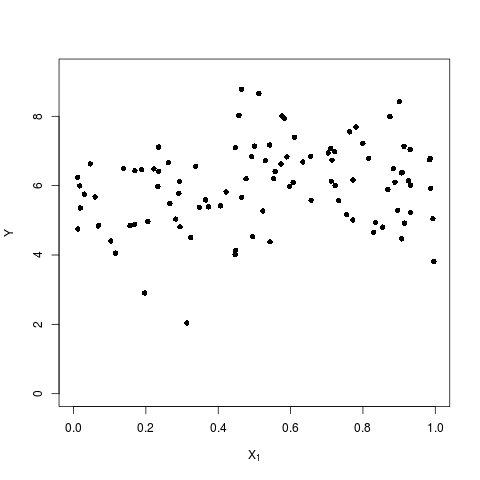
\includegraphics[width = 0.7\textwidth]{./plots/confounding_simple.png}
\end{frame}

\begin{frame}
\frametitle{Multiple regression: motivation}
What do you think the relationship is between $X_1$ and $Y$?

\vspace{-0.3cm}

\centering
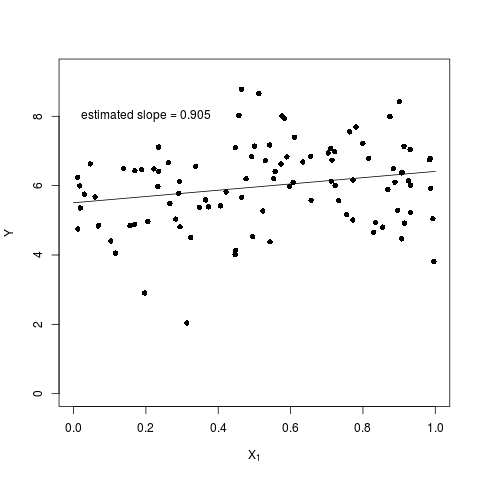
\includegraphics[width = 0.7\textwidth]{./plots/confounding_simple_with_line.png}
\end{frame}

\begin{frame}
\frametitle{Multiple regression: motivation}
How about now?

\vspace{-0.3cm}
\centering
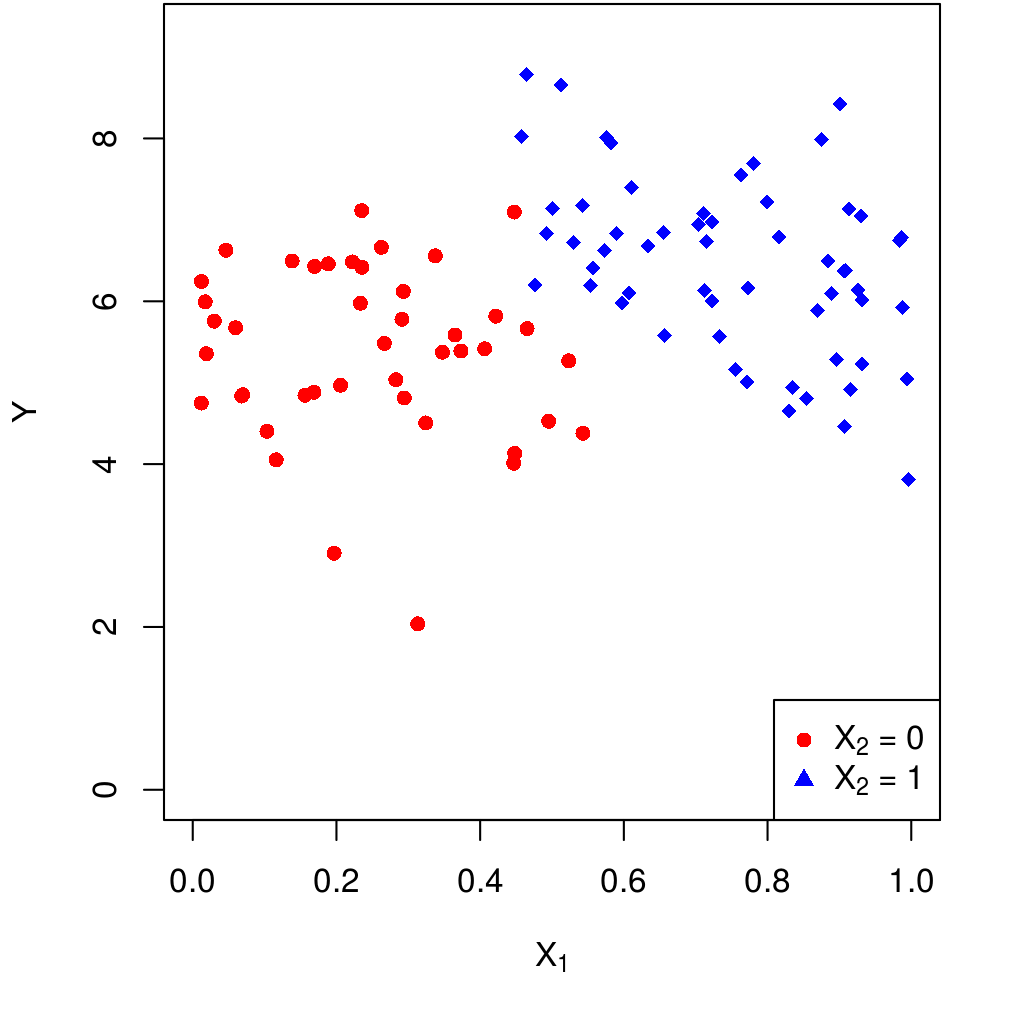
\includegraphics[width = 0.7\textwidth]{./plots/confounding_colored.png}
\end{frame}

\begin{frame}
\frametitle{Multiple regression: motivation}
How about now?

\vspace{-0.3cm}
\centering
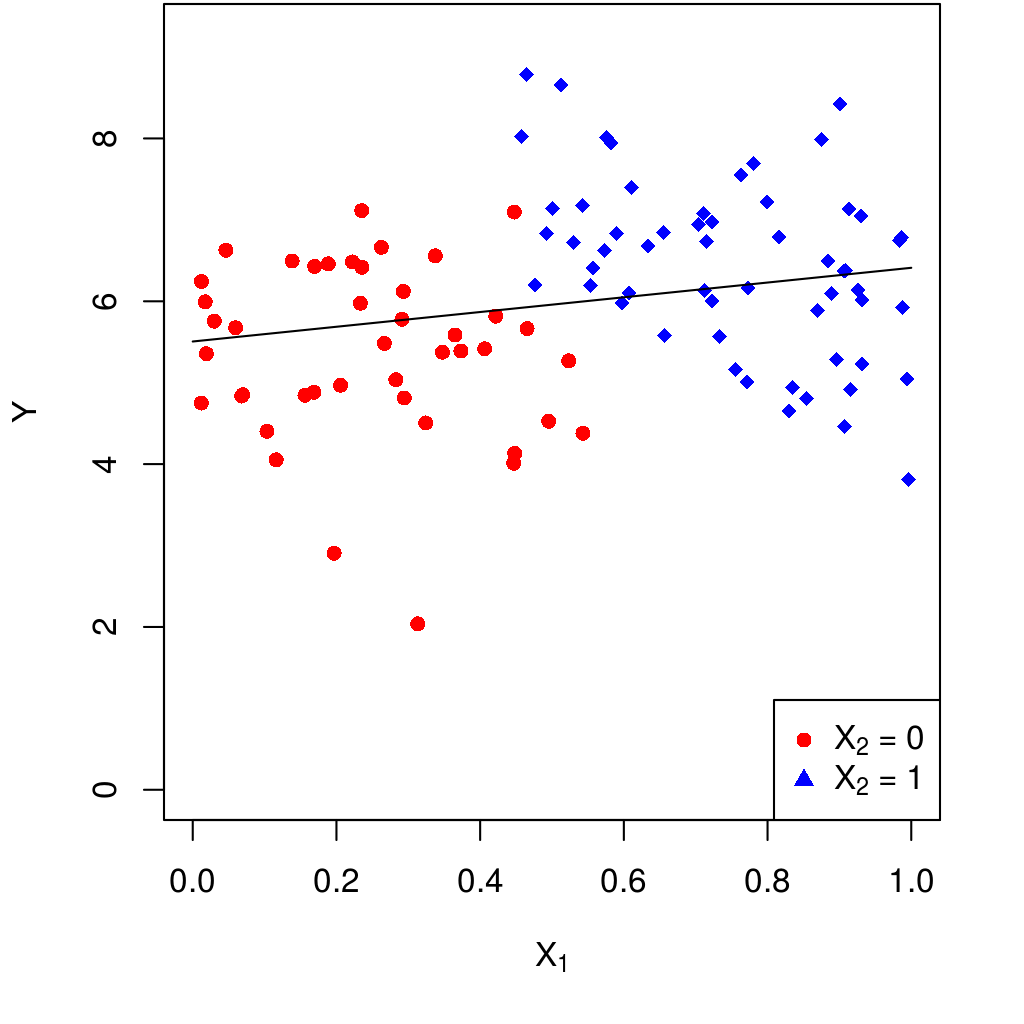
\includegraphics[width = 0.7\textwidth]{./plots/confounding_colored_with_simple_line.png}
\end{frame}

\begin{frame}
\frametitle{Multiple regression: motivation}
How about now?

\vspace{-0.3cm}
\centering
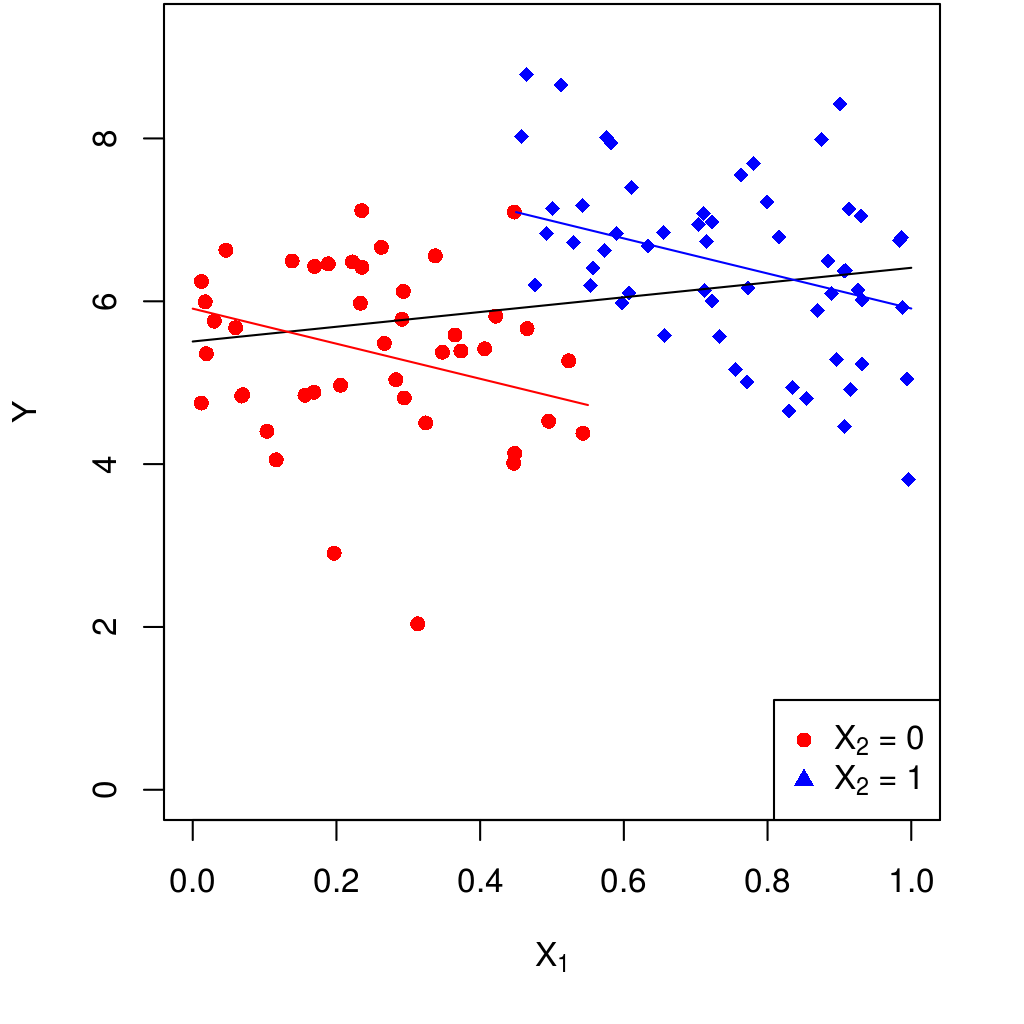
\includegraphics[width = 0.7\textwidth]{./plots/confounding_colored_with_lines.png}
\end{frame}

\begin{frame}
\frametitle{Multiple regression: notation}
\end{frame}

\begin{frame}
\frametitle{Multiple regression: FEV}
\end{frame}


\section{Wrapping up}
\begin{frame}
\frametitle{SECTION 3: WRAPPING UP}
\end{frame}
\end{comment} % end comment block

\end{document}
